\documentclass[runningheads,a4paper]{llncs}

\usepackage{verbatim}
\usepackage{amssymb}
%\usepackage{amsmath} % Used for 'align' environment
\setcounter{tocdepth}{3}
\usepackage{graphicx} % Used for inserting pdf as graphics
\usepackage{float} % Used fo0r 'H' float option in figures
\usepackage{hyperref} % Used for creating a hyperlink to reference parts
\usepackage{enumitem}
\usepackage{textcomp}
\usepackage{multicol}
\usepackage{tikz}
\usepackage[ruled,vlined,linesnumbered]{algorithm2e}
\usetikzlibrary{positioning}
\usetikzlibrary{shapes.multipart}
\usetikzlibrary{shapes.misc} % used for rounded rectangle

\let\proof\relax 
\let\endproof\relax 
\usepackage{amsthm}


\usepackage{multirow}
\usepackage{url}
\usepackage{color}
\urldef{\mailsa}\path|radelacruz@up.edu.ph|
\urldef{\mailsb}\path|fccabarle@up.edu.ph|
\urldef{\mailsc}\path|ivan.cedric10@gmail.com|
\urldef{\mailsd}\path|hnadorna@dcs.upd.edu.ph|
\urldef{\mailse}\path|zxxhust@gmail.com|
\usepackage{mathtools}
\DeclarePairedDelimiter\ceil{\lceil}{\rceil}
\DeclarePairedDelimiter\floor{\lfloor}{\rfloor}
    
\newcommand{\keywords}[1]{\par\addvspace\baselineskip
\noindent\keywordname\enspace\ignorespaces#1}
%\newcommand{\tt}[1]{\texttt{#1}}



\begin{document}

\mainmatter

\title
{
On Homogeneous Spiking Neural P System Variants
}

\titlerunning
{
Homogeneous SNPSP Systems
}


\author
{
Ren Tristan A. de la Cruz$^1$
\and
Francis George C. Cabarle$^{1,2}$
\and
Iva Cedric H. Macababayao$^{1}$
\and
Henry N. Adorna$^1$ 
\and
Xiangxiang Zeng$^3$
}

\authorrunning {de la Cruz et al}


\institute
{
$^1$Algorithms and Complexity Laboratory \\
Department of Computer Science, University of the Philippines - Diliman\\
Diliman 1101, Quezon City, Philippines    \\
$^2$Shenzhen Research Institute of Xiamen University \\
Xiamen University, Shenzhen 518000, Guangdong, China.\\
$^3$ School of Information Science and Engineering\\
Hunan University 410082, Changsha, China \\
\mailsa , \mailsb, \mailsc, \mailsd, \mailse 
}

\newcommand{\ra}{\rightarrow}
\newcommand{\se}{\text{ }}

\toctitle{Lecture Notes in Computer Science}
\tocauthor{Authors' Instructions}


\maketitle

% ================================================================================================= %

\begin{abstract}

(ABSTRACT)

\keywords{Membrane Computing, 
          Spiking Neural P Systems, 
          Homogeneous Neurons,
          Structural Plasticity}
\end{abstract}

% ================================================================================================= %

\section{Introduction}

% ================================================================================================= %


\section{Spiking Neural P System and Some Variants} \label{sec-snps}

% ================================================================================================= %


\section{Homogenization of Spiking Neural P Systems} \label{sec-homo}

\subsection{Representing Neurons as Labelled Transition Systems}

We will use the concept of \emph{labelled transition systems} to represent the activities (usages of
rules, receiving spikes) in a neuron.

\begin{definition}[Labelled Transition System]
A labelled transition system is a tuple $(S, L, \ra)$ where $S$ is a set of states, $L$ is a set of
labels, and $\ra$ is a relation of labelled transitions ($\ra \subseteq S \times L \times S$). 
\end{definition}

In the context of SNP systems, a \emph{state} will be a set of natural numbers that represent a set
of spike counts. For example, the state $\{4,5\}$ represents spike counts $4$ and $5$, the state 
$\{0,2,4,8,...\}$ represents even spike counts, and the state $\{15,20,25,30,35,...\}$ represents 
spike counts that are multiples of $5$ greater that or equal to $15$.

We will use \emph{labels} of the form $(\alpha, \beta)$ where $\alpha$ is an integer while $\beta$ 
represents an action of a rule. In SNP systems, labels with $\alpha<0$ are used for transitions that 
represent events that involve rule usage while labels with $\alpha>0$ are used for transitions that 
represent events that involve reception of spikes. $\beta$ represents an action (e.g. spiking, 
forgetting) of a rule so it value is more relevant to labels with $\alpha < 0$ which represent some
rule usage. For example, in SNP systems that only use standard spiking rules without delay, the
label $(-2,a)$ is associated with a spiking rule that consumes $2$ spikes while the label 
$(-5,\lambda)$ is associated with forgetting rule that consumes $5$ spikes. Labels with $\beta = a$ 
represent spiking rules while labels with $\beta=\lambda$ represent either forgetting rules or 
reception of spikes. Since labels with $\alpha > 0$ represent reception of spikes, if there are
no rule usage involve, we can simply set their $\beta$ components to $\lambda$. For example, the 
label $(+3,\lambda)$ represents the event where the neuron receives $3$ spikes in one step while the 
label $(+2,\lambda)$ represents the event where the neuron receives $2$ spikes.

For label $(\alpha,\beta)$, $\alpha \in \mathbb{Z}$ while $\beta \in \mathcal{A}$ where 
$\mathcal{A}$ is some set of \emph{actions} for a specific SNP system variant. In the previous 
example, $\mathcal{A} = \{a,\lambda\}$ was used for SNP systems that use standard spiking rules 
without delay. For SNP systems with extended spiking rules without delay, the set of actions can be
$\mathcal{A} \subset \mathbb{N}$. $\beta \in \mathcal{A}$ is a natural number that represents the
number of spikes produced by some extended spiking rule. For example, the label $(-3,2)$ can
represent a rule the consumes $3$ spikes and produce $2$ spikes while the label $(-5,0)$ is a 
forgetting rule that consumes $5$ spikes. For an given SNP system variant, the set of labels that 
will be used is some set $L \subseteq \mathbb{Z} \times \mathcal{A}$ where $\mathcal{A}$ is the 
set of actions of the rules associated with the SNP system variant.

A \emph{transition} is a tuple of the form $(S_x, (\alpha,\beta), S_y)$ where $S_x$ and $S_y$ are
states and $(\alpha, \beta)$ is the transition label. The transition $(S_x,(\alpha,\beta),S_y)$ can
also be written as $S_x \xrightarrow[]{(\alpha,\beta)} S_y$. For SNP systems, since $S_x$ and $S_y$
are sets of natural numbers representing sets of spike counts and $(\alpha, \beta)$ represents an
event that might include consumption of spikes and/or reception of spikes, the transition 
$(S_x, (\alpha,\beta),S_y)$ has a particular form. For the transition $(S_x, (\alpha,\beta),S_y)$,
the state $S_y$ is defined in terms of state $S_x$ and the $\alpha$ of the transition label,
$S_y = \{s_x + \alpha\se| \se s_x \in S_x \}$. For example, if $S_x = \{2,4,6,8,...\}$  (set of even 
numbers) and $\alpha = -1$, then $S_y = \{1,3,5,7,...\}$ (set of odd numbers). Due to this 
particular form, we can simply write the transition $(S_x, (\alpha,\beta),S_y)$ as 
$(S_x, (\alpha,\beta))$. The $S_y$ component is already implied. A \emph{transition relation} $\ra$ 
is simply a set of transitions over a given set of states and set of labels.

We will use a labelled transition system to represent activities associated with a neuron. Each 
neuron in the system will have its own transition system representation. 


If a neuron has $n$ spikes, we will say that the neuron \emph{in state $S$} if $n \in S$. For
example, let $n=10$ be the number spikes in the neuron and $S_a=\{1\}$, $S_b=\{2,4,9,10,...\}$, 
$S_c=\{5,10,15,20,...\}$ be states, the neuron is not in state $S_a$ since $n \notin S_a$ but it is
in state $S_b$ and $S_c$ since $n \in S_a$ and $n \in S_b$. States can intersect since they are sets
which means a neuron can be in multiple states at the same time. 


Most states that are associated with a given neuron represent the regular expressions of the rules
in the neuron. For example, in Figure \ref{fig-two-neurons}, neuron $1$ have the rules
$r_1: a/a \ra \lambda$ and  $r_2: a^3(a^2)^*/a^2 \ra a$. The state $S_a=\{1\}$ represents the
regular expression $a$ of rule $r_1$ while the state $S_b=\{3,5,7,9,11,...\}$ represents the regular 
expression $a^3(a^2)^*$ of rule $r_2$. The state $S_c = \{0,2,4,6,8,...\}$, the set of even spike
counts, is also associated with neuron $1$ even though it does not represent a regular expression of
any of the rules in neuron $1$. State $S_c$ is relevant to neuron $1$ because neuron $1$ can be in
state $S_c$. For example, if neuron $1$ starts with $0$ spike and only receives even number of
spikes, then neuron $1$ will stay in state $S_3$.

For neuron $2$ in Figure \ref{fig-two-neurons}, it has the single rule $r_3: a^3/a^3 \ra a$ which 
means $S_z = \{3\}$ is associated with the neuron and it represents the regular expression $a^3$ of 
rule $r_3$. Neuron $2$ only has one incoming synapse so it can only receive one spike at a time 
assuming the use of non-extended/standard spiking rules. The only other relevant states for neuron 
$2$ are $S_w=\{0\}$, $S_x=\{1\}$, $s_y=\{2\}$. If neuron $2$ starts with $0$ spike, it will be state 
$S_w$. Neuron $2$ will be in state $S_x$ after receiving a spike, in state $S_y$ after receiving a 
total of $2$ spikes, and in state $S_z$ after receiving a total of $3$ spikes. At state $S_z$, 
neuron $2$ will use rule $r_3$ consuming $3$ spikes and  returning to state $S_w$. Only states
$S_w, S_x, S_y, S_z$ are relevant to neuron $2$ since it can only reach the spike counts in those
states.

\begin{figure}[H]                                                                                    
\begin{center}                                                                                         
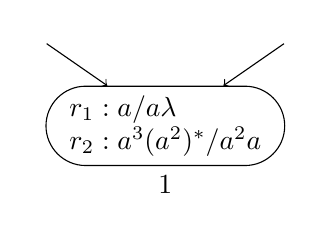
\begin{tikzpicture}                                                                                     
[                                                                                                       
neuron/.style={rounded rectangle, draw, minimum size = 10mm, align=left},                                                      
text-a/.style={black},                                                                                   
]                                                                                                       
\node (n1)   [neuron]                              {$r_1: a/a \ra \lambda$ \\ 
                                                    $r_2: a^3(a^2)^*/a^2 \ra a$};
\node (n1-d) [text-a, below       = 00.00mm of n1] {$1$};                                      
\node (s11)  [text-a, above right = 07.00mm of n1] {};                                      
\node (s12)  [text-a, above left  = 07.00mm of n1] {};
\draw [->]   (s11) -- (n1);                                    
\draw [->]   (s12) -- (n1);                                    
\end{tikzpicture}                                                                                       
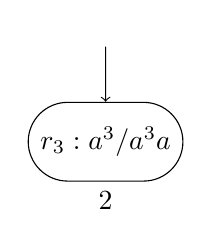
\begin{tikzpicture}                                                                                     
[                                                                                                       
neuron/.style={rounded rectangle, draw, minimum size = 10mm, align=left},                                                      
text-a/.style={black},                                                                                   
]                                                                                                       
\node (n2)   [neuron]                        {$r_3: a^3/a^3 \ra a$};
\node (n2-d) [text-a, below = 00.00mm of n2] {$2$};                                      
\node (s21)  [text-a, above = 07.00mm of n2] {};                                      
\draw [->]   (s21) -- (n2);                                    
\end{tikzpicture}                                                                                       
\end{center}
\caption{Example Neurons}                                                                                            
\label{fig-two-neurons}
\end{figure}                                                                                            

\begin{figure}[H]                                                                                    
\begin{center}                                                                                         
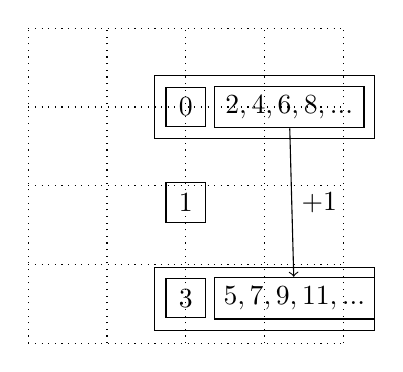
\begin{tikzpicture}
[
state/.style={rectangle, draw, minimum size = 5mm, align=left},                                                      
text-a/.style={black},                                                                                   
]
\draw [dotted] (-3,-3) grid (1,1);
\node (sc)  [state, minimum height = 08.00mm, minimum width = 28mm] at (0,0) {$ $};
\node (sc1) [state] at (-10mm,0) {$0$} ;
\node (sc2) [state, right = 01.00mm of sc1, minimum width = 19mm] {$2,4,6,8,...$}; 
\node (sa) [state, below = 07.00mm of sc1] {$1$};
\node (sb1) [state, below = 07.00mm of sa] {$3$};
\node (sb2) [state, right = 01.00mm of sb1] {$5,7,9,11,...$}; 
\node (sb)  [state, minimum height = 08.00mm, minimum width = 28mm] at (0,-2.44) {$ $};
\path [->] (sc2) edge node [right] {$+1$} (sb2);
\end{tikzpicture}

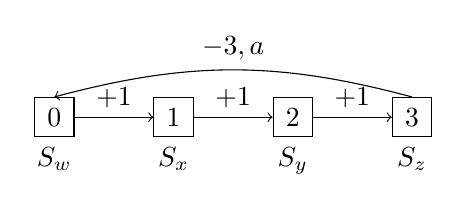
\begin{tikzpicture}                                                                                     
[                                                                                                       
state/.style={rectangle, draw, minimum size = 5mm, align=left},                                                      
text-a/.style={black},                                                                                   
]                                                                                                       
\node (sw)   [state]                              {$0$};
\node (swl)  [text-a, below = 00.00mm of sw]      {$S_w$};
\node (sx)   [state, right = 10.00mm of sw]       {$1$}; 
\node (sxl)  [text-a, below = 00.00mm of sx]      {$S_x$};
\node (sy)   [state, right = 10.00mm of sx]       {$2$}; 
\node (syl)  [text-a, below = 00.00mm of sy]      {$S_y$};
\node (sz)   [state, right = 10.00mm of sy]       {$3$}; 
\node (szl)  [text-a, below = 00.00mm of sz]      {$S_z$};
\draw [->]   (sw) edge node [above] {$+1$} (sx);                                    
\draw [->]   (sx) edge node [above] {$+1$} (sy);                                    
\draw [->]   (sy) edge node [above] {$+1$} (sz);                                    
%\draw [->]   (sz.north) edge [bend right=10] node [auto, swap] {$-3,a$} (sw.north);                                    
\path [->]   (sz.north) edge [bend right=15] node[above] {$-3,a$} (sw.north);                                    
%\draw  [->, bend above]   (sz.north) --  (sw.north);                                    
\end{tikzpicture}                                                                                       
\end{center}
\caption{Example Neurons}                                                                                            
\label{fig-two-state-diagrams}
\end{figure}                                                                                            

%===================================================================================================

\subsection{Operations on Labelled Transition Systems}

\begin{definition}[State Translation]
A state translation is an operation on a state. As a function, it takes a state $S$ and a natural
number $\delta$ and maps it to the state $S'$ defined as $S' = \{s + \delta\se|\se s \in S\}$. We
denote state translation with the $+$ symbol. i.e. $S' = S+\delta = \{s + \delta\se|\se s \in S\}$.
We say that $S'$ is ``$S$ translated by $\delta$".
\end{definition}

For example, let $S=\{3,5,7\}$ and $\delta = 3$, then $S+3 = \{6,8,10\}$. Let $S = \{3,6,9,12,...\}
= \{3i\}_{i\geq 1}$ and $\delta = 1$, then $S+1 = \{4,7,10,13,...\}=\{3i+1\}_{i\geq 1}$.

\begin{definition}[Transition Translation]
A transistion translation is an operation on a transition. The function translate takes a transition
$T = (S,(\alpha,\beta))$ and a natural number $\delta$ and maps it to the transition 
$T' = (S',(\alpha,\beta))$ where $S'=S+\delta$ ($S$ (state) translated by $\delta$). If the context
is clear, we will use the same symbol $+$ for transition translation. i.e. $T' = T +\delta$.
\end{definition}


\begin{definition}[Transition System Translation]
A transition system translation is an operation on an entire transition system. As a function, it
takes a transition system $TS=(S,L,\ra)$ and a natural number $\delta$ and maps them to the 
transition system $TS'=(S',L,\ra')$ where $S'=\{s+\delta\se|\se s \in S\}$ and $\ra' = \{T+\delta
\se|\se T \in \ra\}$.
\end{definition}

\begin{definition}[State Scaling]
State scaling is an operation on a state. As a function, it takes a state $S$ and a natural number
$\delta$ and maps them to the state $S'$ defined as $S' = \{\delta \cdot s\se|\se s\in S\}$. We say
that $S'$ is ``$S$ scaled by $\delta$" and we use the notation $\delta S'$ for $S'$.
\end{definition}

\begin{definition}[Transition Scaling]
Transition scaling is an operation on a transition. As a function, it takes a transition 
$T=(S,(\alpha,\beta))$ and a natural number $\delta$ and maps them to the transition 
$T'=(S',(\alpha',\beta))$ where $S' = \delta S$ and $\alpha' = \delta \alpha$. We say that $T'$
is ``$T$ scaled by $\delta$" and we use the notation $\delta T$ for $T'$.
\end{definition}

\begin{definition}[Transition System Scaling]
\end{definition}

\subsection{Procedures for Homogenizing Neurons' Rule Sets}

\begin{definition}[Matching Transistions]
\end{definition}

\begin{definition}[Non-deterministic State]
\end{definition}

\begin{definition}[Common Transition Set]
\end{definition}



\begin{algorithm}[H]
\SetAlgoLined
\SetKwInput{KwInput}{$TS_1$, $T_2$}
\SetKwInput{KwOutput}{Output}

\KwInput{Transition alphabet, rules}
\KwOutput{Write here the result}

$StateSet \leftarrow \{\}$\;

\While{While condition}
{
   instructions\;
   \eIf{condition}
   {
      instructions1\;
      instructions2\;
   }
   {
      instructions3\;
   }
}
 
\caption{Combining Two Transitions Systems}
\end{algorithm}


% ================================================================================================================================================== %

\bibliographystyle{splncs03}
\bibliography{homonegenous-snp}

\end{document}





























